\documentclass[12pt,letterpaper,titlepage]{article}
\usepackage{solarized-light}
\usepackage{fontspec}
\defaultfontfeatures{Mapping=tex-text}
\usepackage{xunicode}
\usepackage{xltxtra}
\usepackage{amsmath}
\usepackage{pdfpages}
\usepackage{amsfonts}
\usepackage{amssymb}
\setcounter{secnumdepth}{0}
\usepackage{nameref}
\usepackage{enumitem}
\usepackage{environ}
\usepackage{pdfpages}
\usepackage{pgfplots}
\usepackage{karnaugh-map}

\setmainfont{Times New Roman}
\showboxdepth=\maxdimen
\showboxbreadth=\maxdimen


\usepackage{paracol}
\usepackage{wrapfig}
\globalcounter{table}
\globalcounter{figure}
\usepackage{graphicx}
\usepackage[left=1in,right=1in,top=1in,bottom=1in]{geometry}
\graphicspath{{img/}}

\author{Jacob Abel}
\title{	Project 2
	\\\large ECE3544 CRN:82989
}

\setlength{\parskip}{0.25em}

\begin{document}
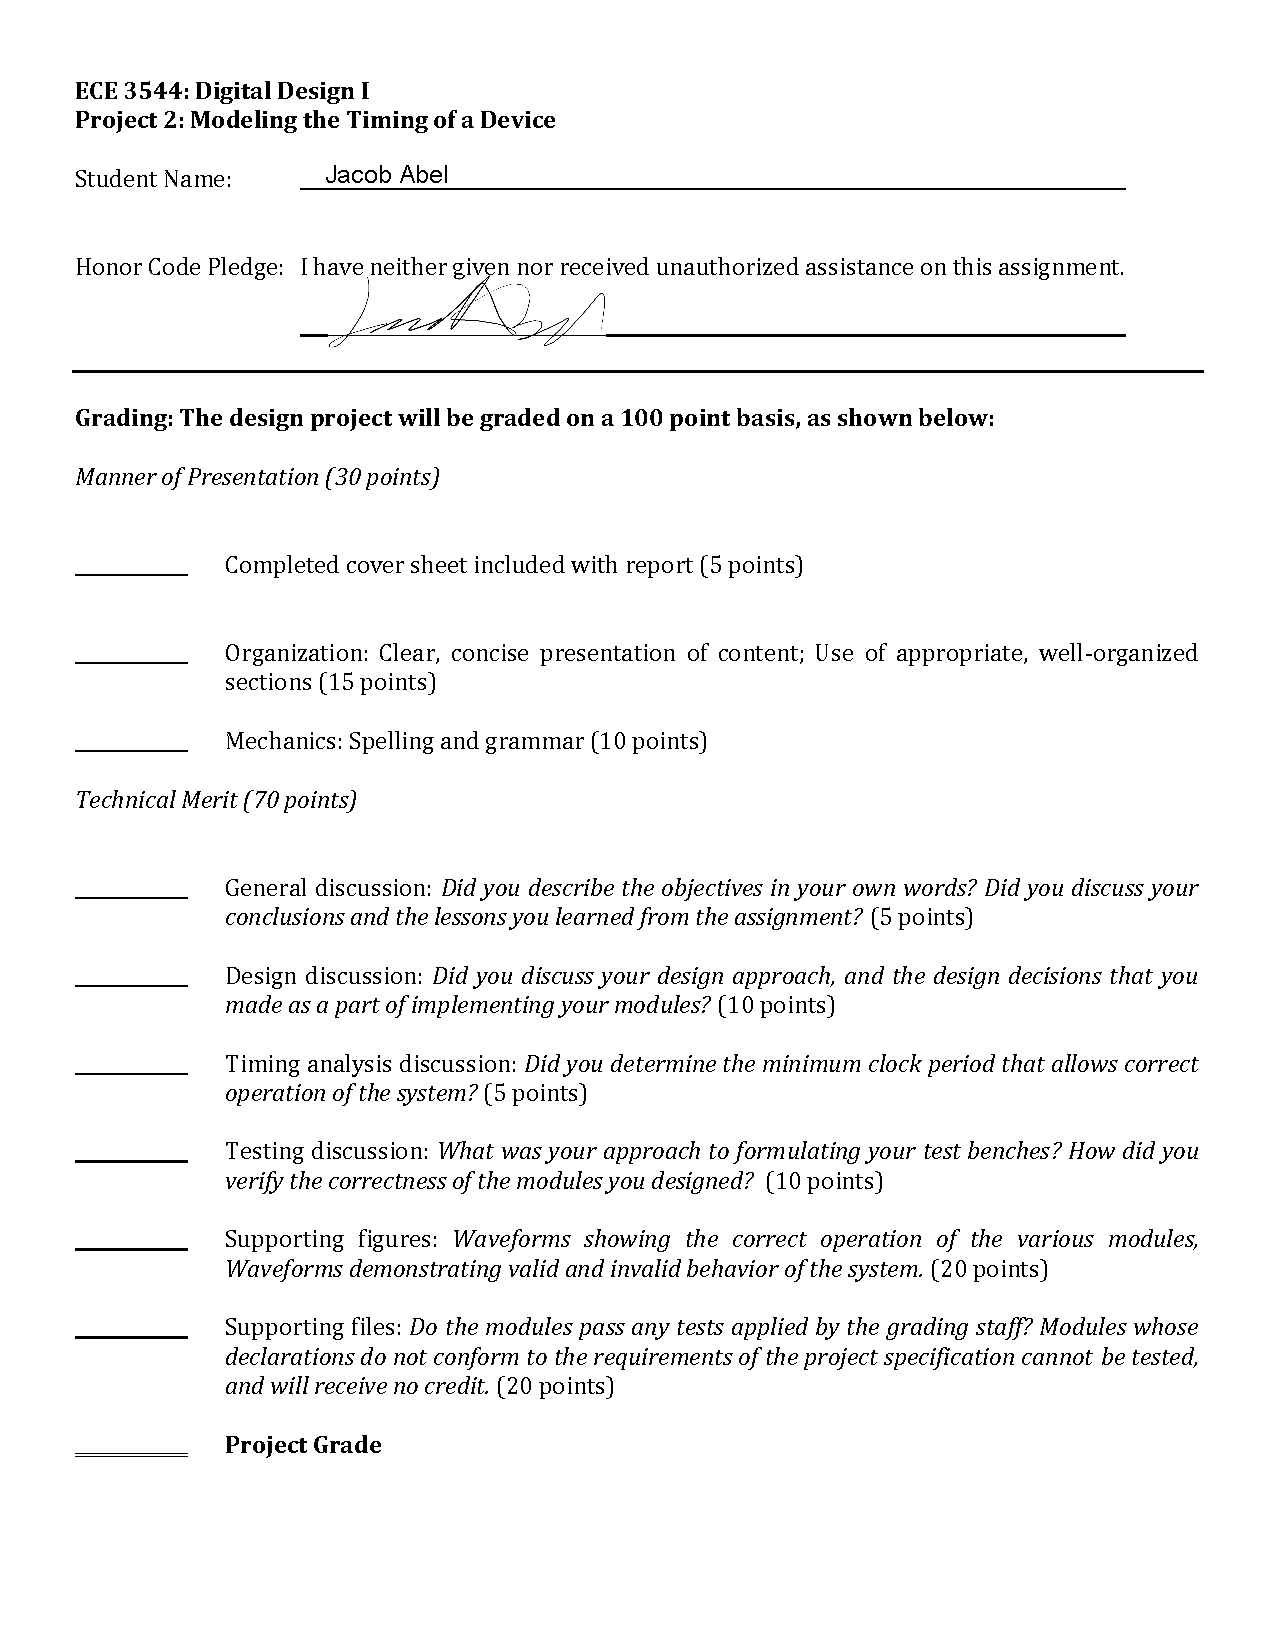
\includepdf[noautoscale]{CoverSheet.pdf}

\maketitle
\begin{raggedright}

\section*{Objective}
The objective of this project is demonstrate basic competence with modelling pre-existing components in Verilog and the ability to analyse a simulated system utilising these components. Additionally, this project demonstrates a capacity to determine the existence of timing errors due to propagation delays.

\section{Comparator Design}

The comparator module compares two 4-bit inputs and a set of cascade inputs in the same manner as the CD74HC85 High Speed CMOS Comparator. The truth table was analysed to determine the various functions required to implement the comparator and then the untimed variant was implemented using behavioural Verilog and nonblocking assignments. The test bench was developed in two parts: the first part demonstrates equivalence to every value in the truth table, the second part performs an exhaustive test across all possible values of the comparator using an 11-bit counter module.

Once the untimed comparator was deemed functionally equivalent to the real component, propagation delays were added using specify blocks. This module was then run against the test bench to demonstrate equivalence to the untimed variant.

\begin{paracol}{3}
\centering
\resizebox{\columnwidth}{!}{
\begin{karnaugh-map}[2][4][1][$Eq$][$GtLt$]
  \minterms{1,3,5,7}
  \autoterms[0]
  \implicant{1}{5}
\end{karnaugh-map}
}

$Eq_o = Eq$
\switchcolumn
\centering
\resizebox{\columnwidth}{!}{
\begin{karnaugh-map}[2][4][1][$Eq$][$GtLt$]
  \minterms{0,2}
  \autoterms[0]
  \implicant{0}{2}
\end{karnaugh-map}
}

$Lt_o = \overline{Gt}\cdot\overline{Eq}$

$Lt_o = \overline{Gt + Eq}$

\switchcolumn
\centering
\resizebox{\columnwidth}{!}{
\begin{karnaugh-map}[2][4][1][$Eq$][$GtLt$]
  \minterms{0,4}
  \autoterms[0]
  \implicantedge{0}{0}{4}{4}
\end{karnaugh-map}
}

$Gt_o = \overline{Lt}\cdot\overline{Eq}$

$Gt_o = \overline{Lt + Eq}$
\end{paracol}
\pagebreak
\section{Secondary Modules Design}

Prior to the development of the HC85 test bench, the provided 4-bit counter was adapted into an otherwise equivalent 11-bit counter module. Little was changed except changing the width of all data elements from 4 to 11-bits.

After the completion of the timed HC85 module and test bench, an untimed Verilog implementation of the 74FCT821 10-bit register was created. This module is functionally equivalent to the real 74FCT821 with the exception of propagation delays and tri-state inputs. The design was relatively painless as the module is essentially a 10-bit register and an always block pinned to the rising edge of the clock.

The final module to be designed was a test bench of a system comprised of the HC85, the 10-bit register, the 11-bit counter, and a clock. The initial variant was created with a clock of 50ns which is plenty sufficient for safely evaluating each stage of the system. The test bench of this system was a simple exhaustive test of all variables. This module was then derived into two variants: \texttt{system\_tb1} which has a clock of 16ns, and \texttt{system\_tb2} which has a clock of 10ns. The clock of \texttt{system\_tb1} was determined by reducing the clock to the greatest propagation delay of HC85 which is the $(\texttt{a\_in, b\_in} \implies \texttt{oa\_lt\_b})$ path. Similarly, the clock of \texttt{system\_tb2} was determined by reducing the clock to just past the greatest propagation delay of the shortest branch of HC85 which is the $(\texttt{ia\_lt\_b}, \texttt{ia\_eq\_b}, \texttt{ia\_gt\_b} \implies \texttt{oa\_lt\_b}, \texttt{oa\_gt\_b})$ path.

\pagebreak
\subsection*{Design Process Reflection}

The design process for this project was relatively standard: read all documentation, draft a plan of attack/divide into tasks, and completing \& validating every stage of the project. No single module was all that complex and therefore completing each stage was relatively short and painless. Only two real issues arose. One issue was a scheduling mistake resulting in no time to work on the assignment up until fairly close to the deadline. 

The other issue was that the project required that the HC85 module be implemented in behavioural Verilog which results in a more convoluted and complex design than simply using data flow Verilog. This is largely because the HC85 is combinational and therefore can be reduced into a rather simple set of boolean algebra functions. Below is the alternative data flow variant which is functionally equivalent and much cleaner.
\begin{center}
\centering
\begin{lstlisting}
module hc85(
    input [3:0] a_in, b_in,
    input  ia_lt_b, ia_eq_b, ia_gt_b,
    output oa_lt_b, oa_eq_b, oa_gt_b
);
    specify
        (a_in, b_in => oa_lt_b) = (16);
        (a_in, b_in => oa_gt_b) = (16);
        (a_in, b_in => oa_eq_b) = (14);
        (ia_lt_b, ia_eq_b, ia_gt_b => oa_lt_b) = (11);
        (ia_lt_b, ia_eq_b, ia_gt_b => oa_gt_b) = (11);
        (ia_gt_b => oa_eq_b) = (9);
    endspecify
    wire cmp_lt, cmp_gt, cmp_eq, cas_lt, cas_gt, cas_eq;

    assign cmp_eq = (a_in == b_in);
    assign cmp_gt = (a_in >  b_in);
    assign cmp_lt = (a_in <  b_in);

    assign cas_eq = ia_eq_b;
    assign cas_gt = ~(ia_lt_b || ia_eq_b);
    assign cas_lt = ~(ia_gt_b || ia_eq_b);

    assign oa_eq_b = (cmp_eq && cas_eq);
    assign oa_gt_b = (cmp_gt || (cmp_eq && cas_gt));
    assign oa_lt_b = (cmp_lt || (cmp_eq && cas_lt));

endmodule
\end{lstlisting}

Alternative Data Flow hc85.v
\end{center}

\clearpage
\section{Untimed Comparator Simulation}
\begin{center}
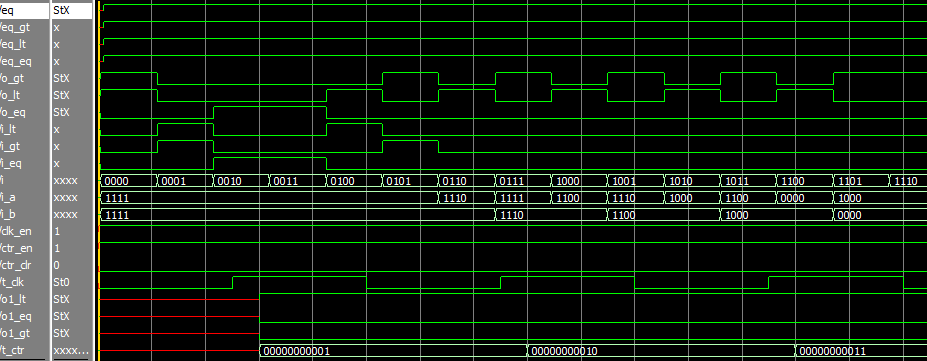
\includegraphics[width=\textwidth]{tb_ut_red}
Truth Table Test
\end{center}

This simulation demonstrates that all the inputs listed on the data sheet result in the correct outputs. The \texttt{i\_a}, \texttt{i\_b}, \texttt{i\_gt}, \texttt{i\_eq}, and \texttt{i\_lt} values are the inputs and the \texttt{o\_gt}, \texttt{o\_eq}, and \texttt{o\_lt} values are the outputs. The \texttt{eq\_} wires demonstrate equivalence on each output pin and the \texttt{eq} wire demonstrates equivalence on all outputs. The equivalences are computed using an XNOR against expected results.

\begin{center}
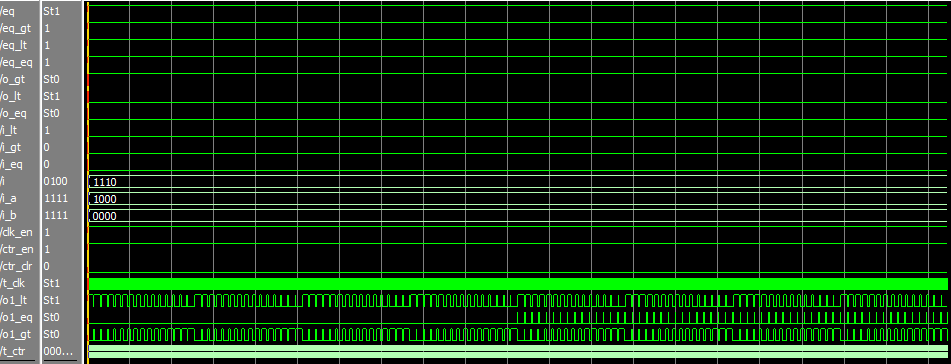
\includegraphics[width=\textwidth]{tb_ut_exh}
Exhaustive Test
\end{center}

Above is the full exhaustive test of the untimed HC85 comparator. The outputs of the exhaustive test are prefixed with \texttt{o1\_}. While all the individual values are not visible, based on the patterns in the waveforms visible from this scale and the results of the truth table test, we can infer that the waveform is correct across all values. The visible patterns such as the mirroring between \texttt{o1\_lt} and \texttt{o1\_gt}, their periodic nature, and that \texttt{o1\_eq} only starts in the second half all mimic the expected behaviour of the comparator.

\clearpage

\section{Timed Comparator Simulation}
\begin{center}
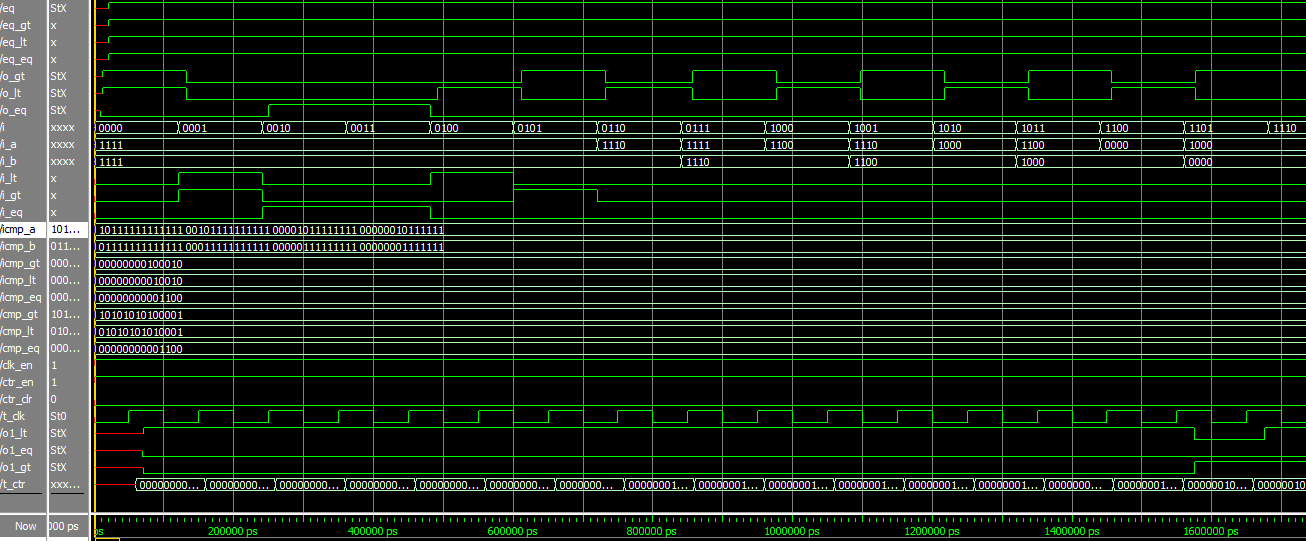
\includegraphics[width=\textwidth]{tb_red}
Truth Table Test
\end{center}

\begin{center}
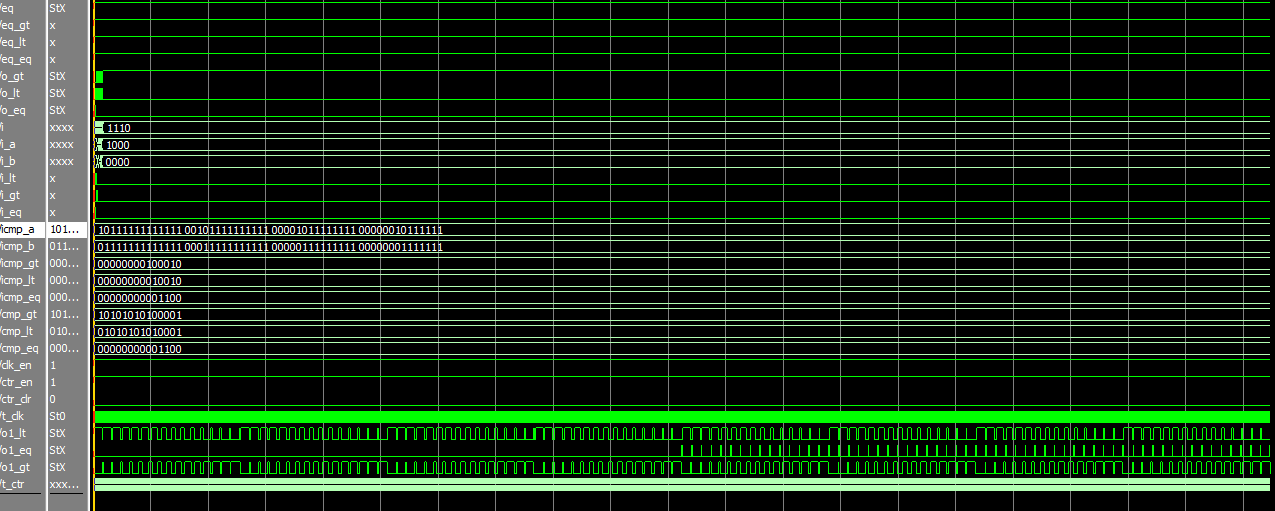
\includegraphics[width=\textwidth]{tb_exh}
Exhaustive Test
\end{center}

The above simulation results are identical to the untimed variant's simulation results with the exception of propagation delay slightly shifting outputs forward. The truth table results are sufficiently zoomed in to be able to verify the propagation delays are correct. The transitions at 250ns, 492ns, and 857ns are 9ns, 11ns, and 16ns respectively. The 14ns transition occurs at 104074ns however it is not visible on the zoomed in simulation results.
\clearpage

\section{Register Simulation}
\begin{center}
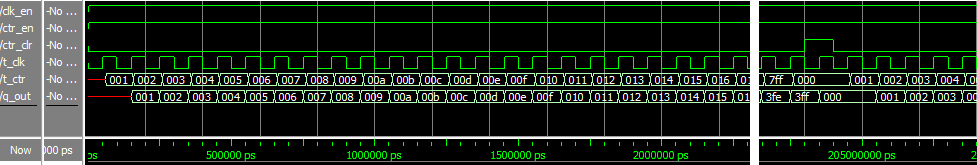
\includegraphics[width=\textwidth]{tb_reg}
Register Simulation
\end{center}

These simulation results demonstrate functionality of the register's parallel load on a rising clock across all 10-bits.

\section{Properly Timed System Simulation}
\begin{center}
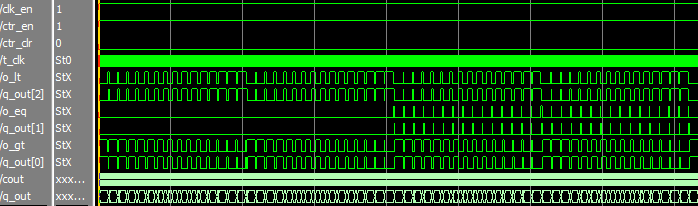
\includegraphics[width=\textwidth]{tb_sys1}
System 1 Simulation
\end{center}

These simulation results show that the outputs are properly being stored and the system is functioning properly at the maximum clock speed.

\pagebreak

\section{Improperly Timed System Simulation}
\begin{center}
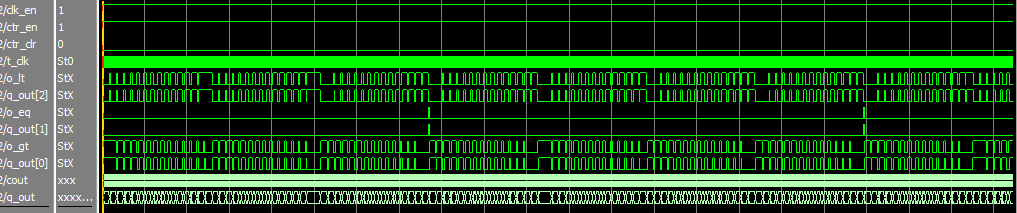
\includegraphics[width=\textwidth]{tb_sys2}
System 2 Simulation
\end{center}
\begin{center}
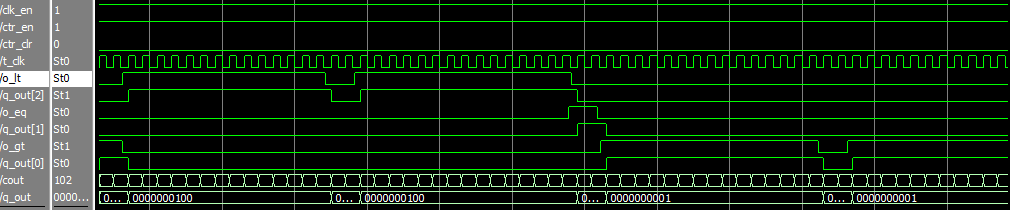
\includegraphics[width=\textwidth]{tb_sys2_2}
System 2 Simulation Close Up 
\end{center}

These simulation results show that the outputs are not being properly stored and the system has exceeded the maximum clock speed. The erratic nature of the output waveform and the staggered overlapping outputs are evidence of this.


\section{Conclusion}

This project demonstrated the effectiveness of Verilog in modelling real world components for simulation and analysis. Additionally it demonstrated the capacity of Verilog simulations in diagnosing timing errors and verifying the timing bounds of the simulated models. Despite starting this project late, the project went remarkably smoothly and very little of the time was spent debugging. As such the project can easily be considered a success with the exception of the scheduling failure that resulted in it being started late.

\end{raggedright}
\end{document}
